\documentclass{article}
\usepackage[utf8]{inputenc}
\usepackage[spanish]{babel}
\usepackage{listings}
\usepackage{graphicx}
\graphicspath{ {images/} }
\usepackage{cite}

\begin{document}

\begin{titlepage}
    \begin{center}
        \vspace*{1cm}
            
        \Huge
        \textbf{Analisis y diseño}
            
        \vspace{0.5cm}
        \LARGE
        Parcial 2
            
        \vspace{1.5cm}
        \textbf{Miguel Angel Serna Montoya}
            
        \vfill
            
        \vspace{0.8cm}
            
        \Large
        Departamento de Ingeniería Electrónica y Telecomunicaciones\\
        Universidad de Antioquia\\
        Medellín\\
        Septiembre de 2021
            
    \end{center}
\end{titlepage}

\tableofcontents

\section{Análisis problema} \label{contenido}
1er día: Por el momento mis ideas algorítmicamente hablando son casi nulas por no decir obsoletas ya que no he podido dedicarle el merecido tiempo al planteamiento del problema. Por el momento me estoy encargando de entender bien los requisitos y restricciones con los que me veo comprometido.
2do día: Me doy cuenta viendo la repetición de la clase que el principal desafió es el de desarrollar las funciones de submuestreo o sobremestrueo. Planeo implementarlas dentro de una clase llamada escalado, esta se incluirá en otra clase llamada 
\section{Consideraciones}
No puedo usar las librerías para el submuestreo o sobremestrueo. Todo tiene que ser de mi puño y letra.
\section{Diseño algoritmo}
\section{Esquema de tareas}
\begin{figure}[h]
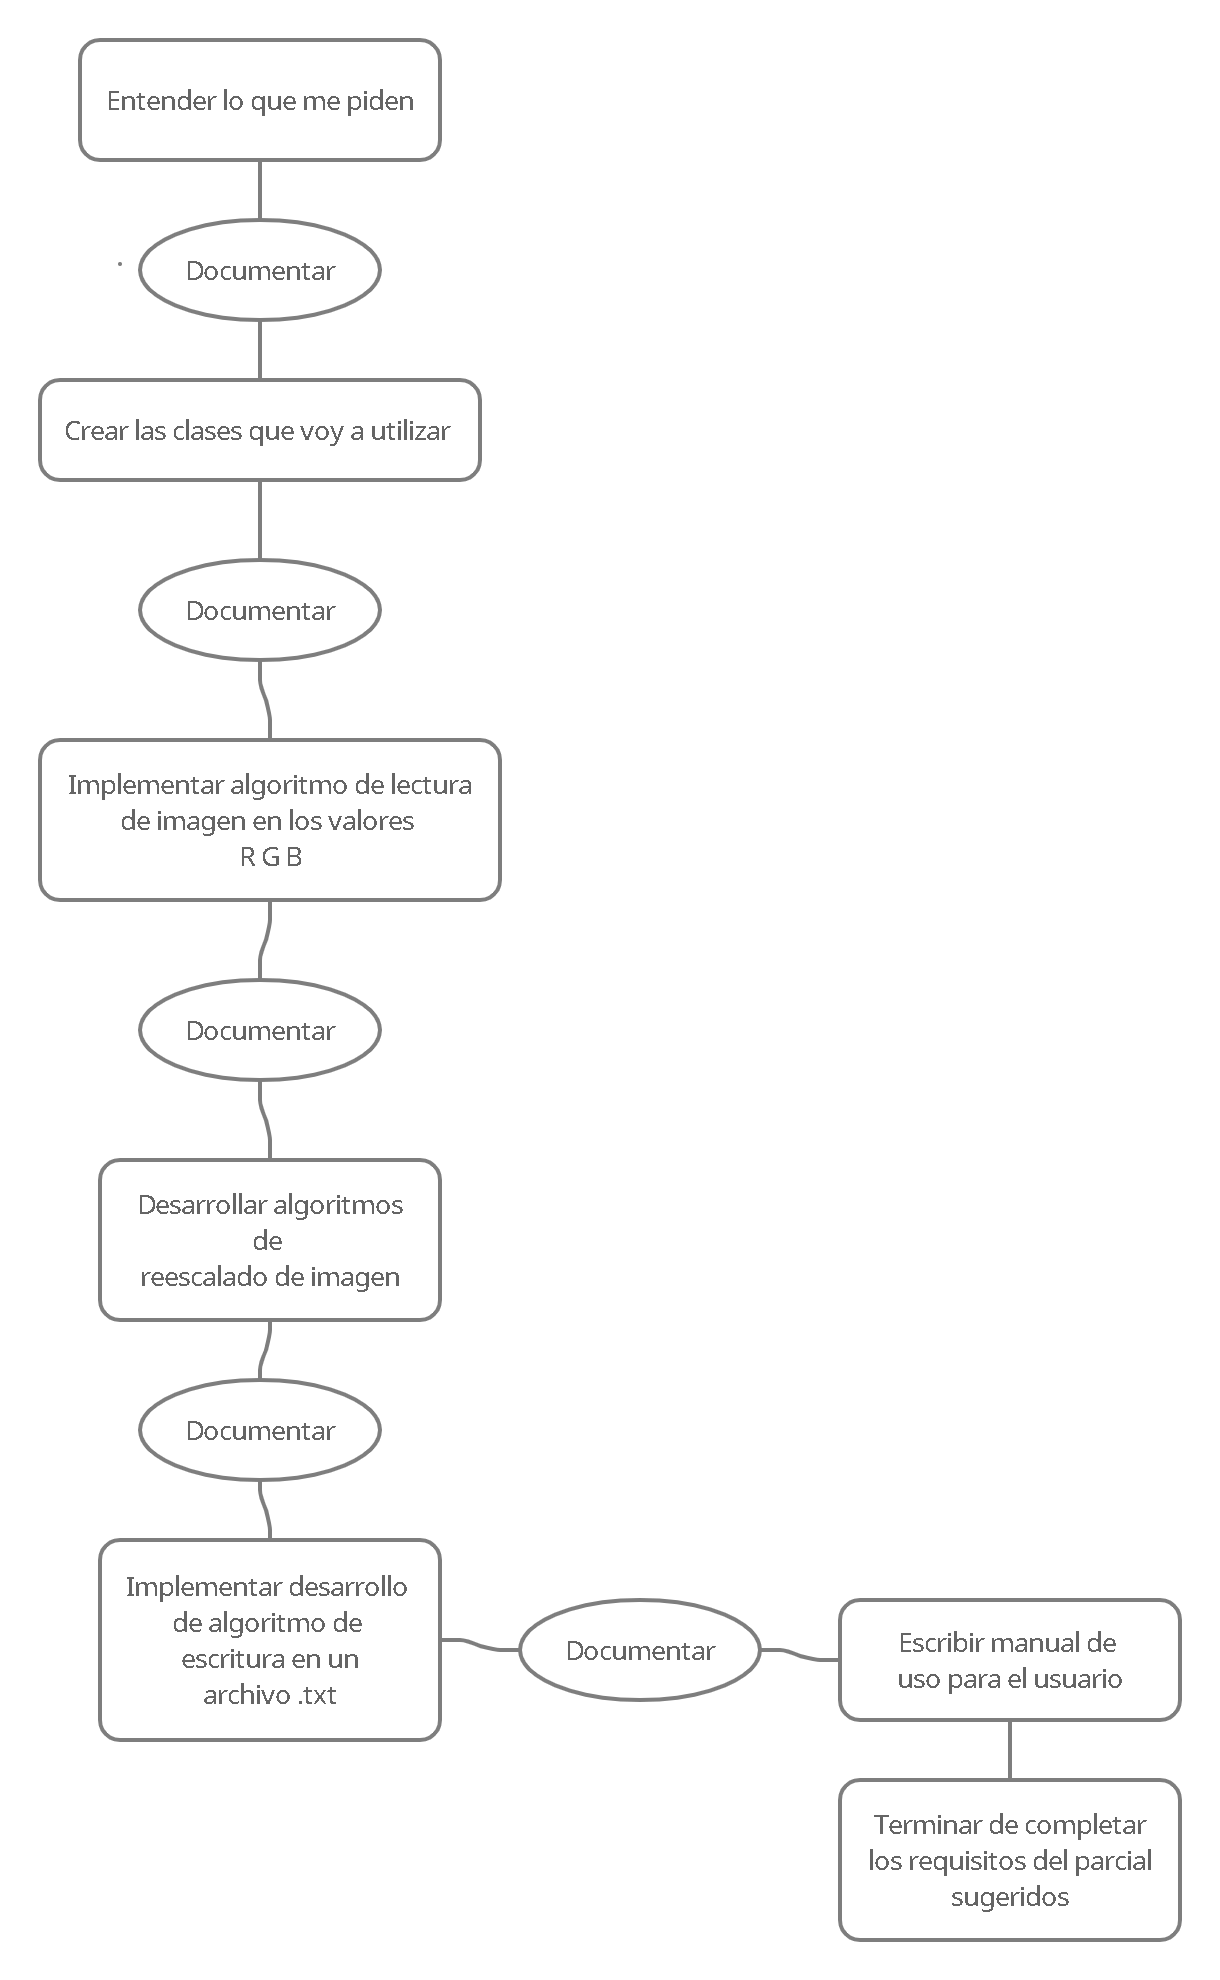
\includegraphics[width=13cm]{imag-analisis/esquema.png}
\centering
\caption{esquema}
\label{fig:pixhell}
\end{figure}


\end{document}